\documentclass[landscape]{exam}

\usepackage{2in1, lscape} 
\usepackage{units} 
\usepackage[fleqn]{amsmath}
\usepackage{float}
\usepackage{mdwlist}
\usepackage{booktabs}
\usepackage{caption}
\usepackage{fullpage}
\usepackage{enumerate}
\usepackage{graphicx}

\printanswers

\everymath{\displaystyle}

\printanswers

\title{Statistics \\ Week Four}
\date{\today}
\author{}

\begin{document}

\maketitle
\tableofcontents

  \section{Homework}

  \begin{itemize*}
    \item TO DO
  \end{itemize*}

  \section{Regression}

  \begin{figure}[H]
    \centering
    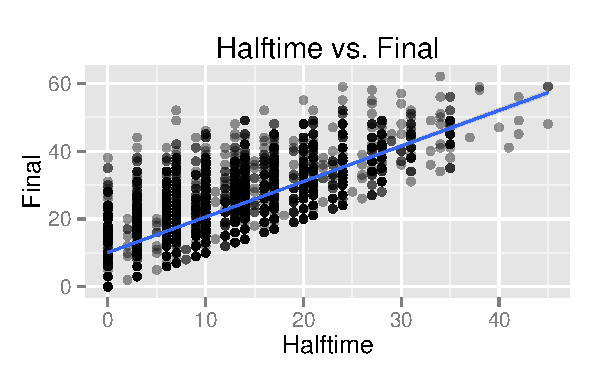
\includegraphics{figures/nfl/ht_vs_final.pdf}
    \caption{Halftime vs. Final Score}
  \end{figure}

  \begin{figure}[H]
    \centering
    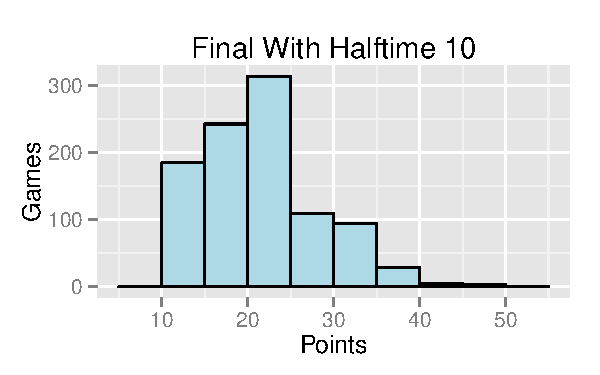
\includegraphics{figures/nfl/ht_10_final.pdf}
    \caption{Final score with a halftime score of 10}
  \end{figure}

  \begin{figure}[H]
    \centering
    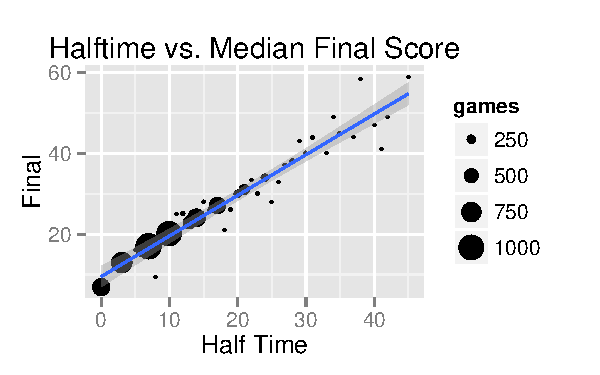
\includegraphics{figures/nfl/ht_vs_median_final.pdf}
    \caption{Halftime vs. Median Final Score}
  \end{figure}

  \begin{figure}[H]
    \centering
    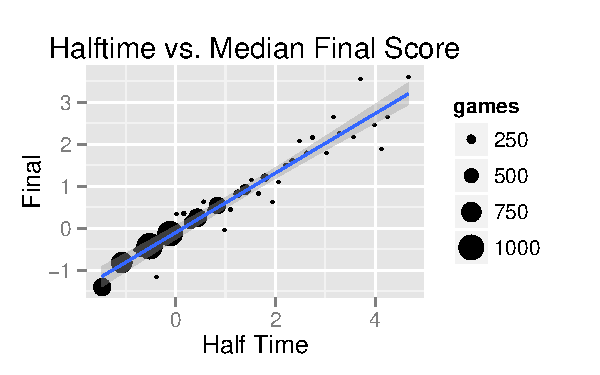
\includegraphics{figures/nfl/ht_vs_median_final_scaled.pdf}
    \caption{Halftime vs. Median Final (scaled)}
  \end{figure}

  \begin{table}[H]
    \centering
    \begin{tabular}{rrrrr}
      \toprule
      \midrule
      Halftime & Mean Final & Halftime s & Final s & slope\\
      0        & 9.53       & -1.48      & -1.15   & NA \\
      3        & 13.06      & -1.07      & -0.81   & 0.83 \\
      7        & 17.76      & -0.53      & -0.36   & 0.83 \\
      10       & 20.96      & -0.12      & -0.05   & 0.75 \\
      14       & 24.61      & 0.43       & 0.30    & 0.64 \\
      17       & 27.81      & 0.84       & 0.61    & 0.75 \\
      \bottomrule
    \end{tabular}
    \caption{Common halftime scores}
  \end{table}

  \begin{tabular}[H]{rr}
    \toprule
    Min Games & Mean Slope $ $r$ \\
    \midrule
    500       & 0.76 \\
    100       & 0.73 \\
    1         & 0.84 \\
    \bottomrule
  \end{tabular}

\end{document}

